
\documentclass[
	12pt, % Default font size, values between 10pt-12pt are allowed
	%letterpaper, % Uncomment for US letter paper size
	%spanish, % Uncomment for Spanish
]{fphw}


% Template-specific packages
\usepackage[utf8]{inputenc} % Required for inputting international characters
\usepackage[T1]{fontenc} % Output font encoding for international characters
\usepackage{mathpazo} % Use the Palatino font
\usepackage{amsmath}
\usepackage{graphicx} % Required for including images
\usepackage{float}
\usepackage{booktabs} % Required for better horizontal rules in tables
\usepackage{textcomp}
\usepackage{listings} % Required for insertion of code

\usepackage{enumerate} % To modify the enumerate environment
\usepackage[framed,numbered,autolinebreaks,useliterate]{mcode}

%----------------------------------------------------------------------------------------
%	ASSIGNMENT INFORMATION
%----------------------------------------------------------------------------------------

\title{Homework \#1} % Assignment title

\author{Le Yang 1751894} % Student name

\date{March 28th, 2025} % Due date

\institute{Tongji University \\ School of Software Engineering} % Institute or school name

\class{Digital Image Processing (42033501)} % Course or class name

\professor{Dr. Qingjiang Shi} % Professor or teacher in charge of the assignment

%----------------------------------------------------------------------------------------

\makeatletter
\renewcommand{\section}{\@startsection{section}{1}{0mm}
  {-\baselineskip}{0.5\baselineskip}{\bf\leftline}}
\makeatother
\begin{document}


\maketitle % Output the assignment title, created automatically using the information in the custom commands above

%----------------------------------------------------------------------------------------
%	ASSIGNMENT CONTENT
%----------------------------------------------------------------------------------------

\section*{1. Denosing for Astrophotography}

\begin{problem}
	a) To generate a single denoised image from each video, compute a running average of the frames $f^t$(t = 1, 2, ...) in the video without frame alignment, according to the following update rule:
	\begin{align*}
		&f^1_{average}=f^1 \\
		&f^1_{average}=\frac{t-1}{t}f^{t-1}_{average}+\frac{1}{t}f^t
	\end{align*}
	Display and submit $f^t_{average}$ at $t=30$ for each video. Comment on how effectively the noise is reduced and how
	much the sharp features are blurred by the averaging operation. 
\end{problem}



\begin{figure}[H]
 
	\centering
	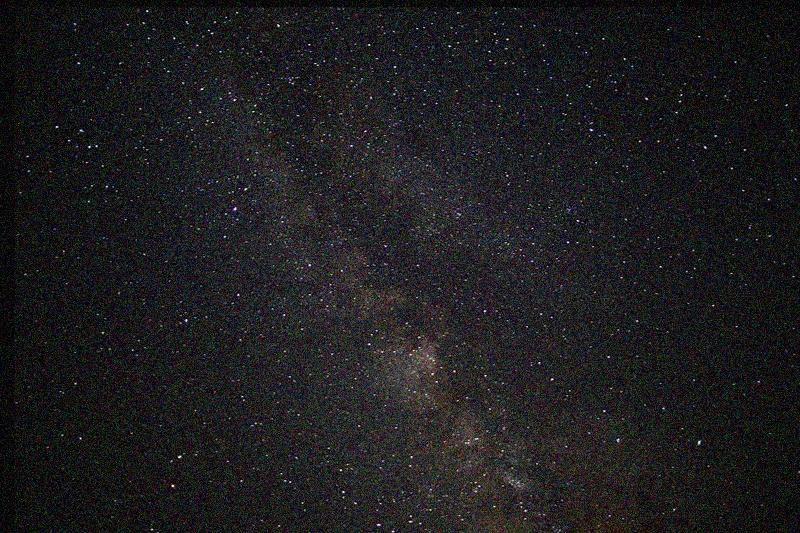
\includegraphics[width=1\columnwidth]{T1/result/sky1origin_30.jpg} % Example image
	\caption{origin 30rd frame of sky\underline{\hspace{0.5em}}1}
	\label{fig1}
\end{figure}
\begin{figure}[H]
 
	\centering
	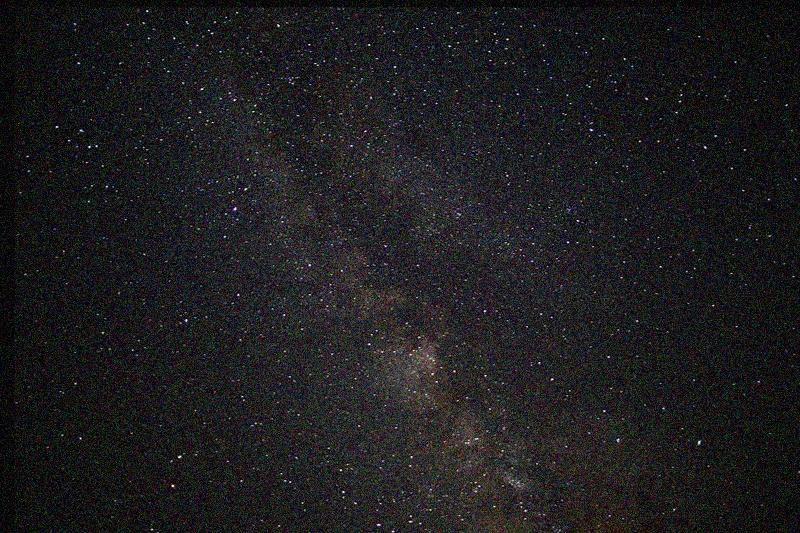
\includegraphics[width=1\columnwidth]{T1/result/sky2origin_30.jpg} % Example image
	\caption{origin 30rd frame of sky\underline{\hspace{0.5em}}2}
	\label{fig2}
	 
\end{figure}


	
%------------------------------------------------

\paragraph*{Answer:}
First, I generate the two origin 30rd frames of the two videos for comparision.The corresponding Matlab code is \textbf{origin.m}. This code generate two images: \textbf{sky1origin\underline{\hspace{0.5em}}30.jpg}, \textbf{sky2origin\underline{\hspace{0.5em}}30.jpg}. They are shown as \textbf{Figure 1} and \textbf{Figure 2}.\\
Then I use the update rule in the question to denoise the image. My Matlab code is followed and is saved as \textbf{without\underline{\hspace{0.5em}}align.m}, this code generate two $f^t_{average}$ at 30rd frame of each video which are shown as \textbf{Figure 3} and \textbf{Figure 4} below. 
\begin{lstlisting}
	%without_align.m
	clc,clear;
	vidobj_1=VideoReader("hw1_sky_1.avi");
	numFrames_1=vidobj_1.NumberOfFrames;
	
	vidobj_2=VideoReader("hw1_sky_2.avi");
	numFrames_2=vidobj_2.NumberOfFrames;
	
	for i=1:numFrames_1
		frame_1=im2double(read(vidobj_1,i));
		image_name_1=strcat('result\sky1woalign_',num2str(i));
		image_name_1=strcat(image_name_1,'.jpg');
		
		frame_2=im2double(read(vidobj_2,i));
		image_name_2=strcat('result\sky2woalign_',num2str(i));
		image_name_2=strcat(image_name_2,'.jpg');
		if(i==1)
			f_average_1=frame_1;
			f_average_2=frame_2;
		else
			f_average_1=(i-1)/i*f_average_1+frame_1/i;
			f_average_2=(i-1)/i*f_average_2+frame_2/i;
		end
		
		if(i==30)
			woalign_1=f_average_1;
			imwrite(woalign_1,image_name_1,'jpg');
			woalign_2=f_average_2;
			imwrite(woalign_2,image_name_2,'jpg');
			break;
		end
	end
\end{lstlisting}
\begin{figure}[H]
 
	\centering
	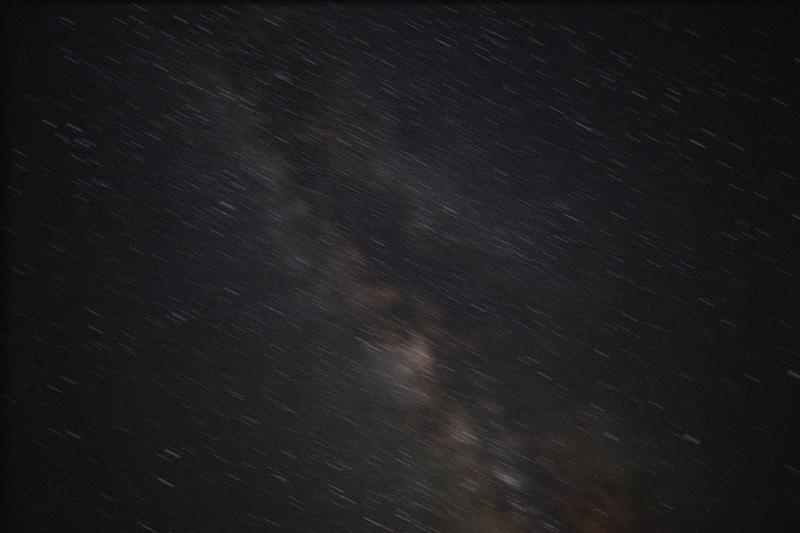
\includegraphics[width=1\columnwidth]{T1/result/sky1woalign_30.jpg} % Example image
	\caption{$f^t_{average}$ at 30rd frame of sky\underline{\hspace{0.5em}}1}
	\label{fig3}
	 
\end{figure}

\begin{figure}[H]
 
	\centering
	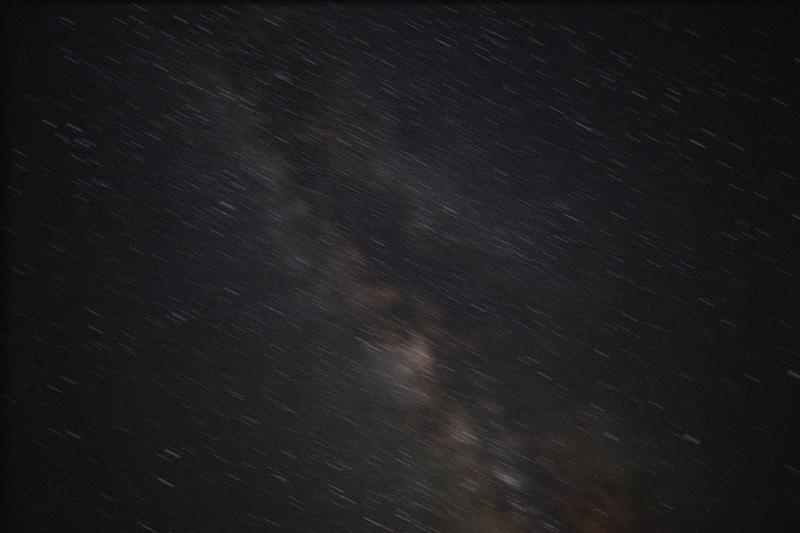
\includegraphics[width=1\columnwidth]{T1/result/sky2woalign_30.jpg} % Example image
	\caption{$f^t_{average}$ at 30rd frame of sky\underline{\hspace{0.5em}}2}
	\label{fig4}
	 
\end{figure}
From the results above, we can see that we reduces the noise in the video to some extent by computing the running average of the frames. It is more easy to recognize in the sky2 video with the moon in the sky because the noise spots mix with stars in the sky1 video. Compared to \textbf{Figure 2}, we can see that in \textbf{Figure 4}, all the noise spots around the moon are removed. However, because we don't utilize frame alignment, we can that many sharp features are blurred by the averaging operation like the edges of the moon in sky2 and stars in sky1. As a result, it is hard to see some details.
%----------------------------------------------------------------------------------------

\begin{problem}
	b)  Now, compute a running average of the frames with frame alignment, according to the following update rule:
	\begin{align*}
		&f^1_{average}=f^1 \\
		&f^1_{average}=\frac{t-1}{t}f^{t-1}_{average}+\frac{1}{t}Align(f^t, f^{t-1}_{average}, t=2,3,\dots
	\end{align*}
	Display and submit $f^t_{average}$ at $t=30$ for each video. Compare to the result in (a) and comment on how effectively noise is reduced while sharp features are better preserved.
\end{problem}


%------------------------------------------------

\paragraph*{Answer:}I use the update rule in the question to denoise the image with frame alignment. My Matlab code is followed and is saved as \textbf{with\underline{\hspace{0.5em}}align.m}, this code generate two $f^t_{average}$ at 30rd frame of each video which are shown as \textbf{Figure 5} and \textbf{Figure 6} below.
\begin{lstlisting}
	%with_align.m
	clc,clear;
	vidobj_1=VideoReader("hw1_sky_1.avi");
	numFrames_1=vidobj_1.NumberOfFrames;
	
	vidobj_2=VideoReader("hw1_sky_2.avi");
	numFrames_2=vidobj_2.NumberOfFrames;
	
	for i=1:numFrames_1
		frame_1=im2double(read(vidobj_1,i));
		image_name_1=strcat('result\sky1wialign_',num2str(i));
		image_name_1=strcat(image_name_1,'.jpg');
		frame_2=im2double(read(vidobj_2,i));
		image_name_2=strcat('result\sky2wialign_',num2str(i));
		image_name_2=strcat(image_name_2,'.jpg');
		if(i==1)
			f_average_1=frame_1;
			f_average_2=frame_2;
		else
			f_average_1=(i-1)/i*f_average_1+Align(frame_1,f_average_1)/i;
			f_average_2=(i-1)/i*f_average_2+Align(frame_2,f_average_2)/i;
		end
		
		if(i==30)
			wialign_1=f_average_1;
			imwrite(wialign_1,image_name_1,'jpg');
			wialign_2=f_average_2;
			imwrite(wialign_2,image_name_2,'jpg');
			break;
		end
	end
\end{lstlisting}
\begin{lstlisting}
	%Align.m
	function aligned = Align(f,g)
	%ALIGN 此处显示有关此函数的摘要
	%   此处显示详细说明
	search = 10;
	minMSE = Inf;
	[height, width, channels] = size(f);
	for dx = -search:search
		for dy = -search:search
			A=[1 0 0
			0 1 0
			dx dy 1];
			tform = maketform('affine', A);
			frameTform = zeros(size(f));

			frameTform = imtransform(f, tform,'bilinear','XData', [1 width], 'YData', [1 height], 'FillValues', zeros(channels,1));


			% Calculates the MSE
			mse = norm( reshape(frameTform, [], 1) - reshape(g, [], 1));
			
			if(mse < minMSE)
			minMSE = mse;
			aligned = frameTform;
			
			end
		end
	end
	end
\end{lstlisting}
\begin{figure}[H]
 
	\centering
	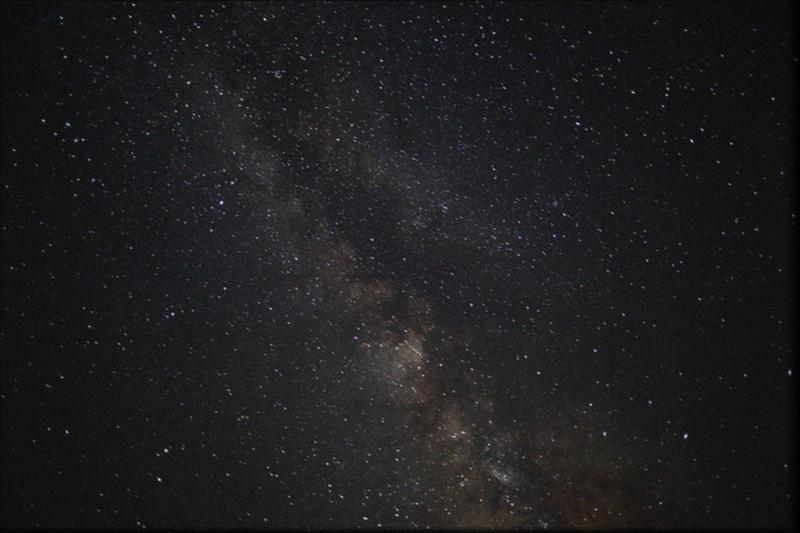
\includegraphics[width=1\columnwidth]{T1/result/sky1wialign_30.jpg} % Example image
	\caption{$f^t_{average}$ at 30rd frame of sky\underline{\hspace{0.5em}}1}
	\label{fig5}
	 
\end{figure}

\begin{figure}[H]
 
	\centering
	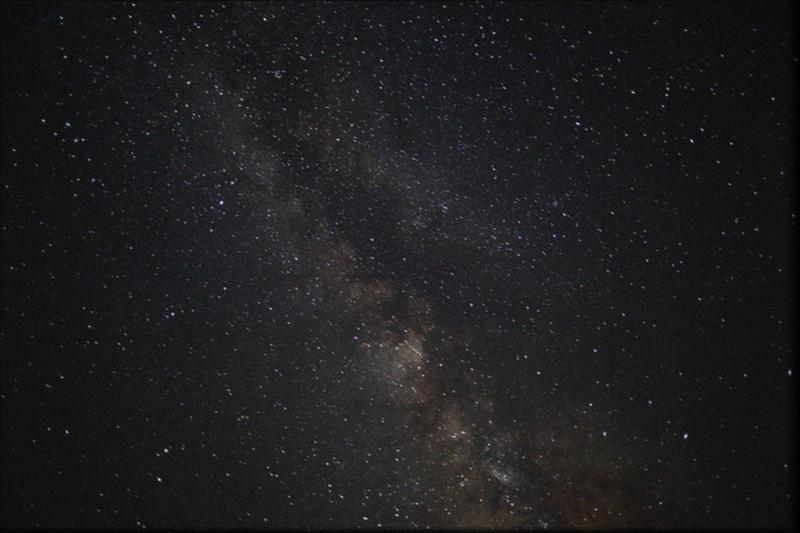
\includegraphics[width=1\columnwidth]{T1/result/sky2wialign_30.jpg} % Example image
	\caption{$f^t_{average}$ at 30rd frame of sky\underline{\hspace{0.5em}}2}
	\label{fig6}
	 
\end{figure}
From the results above, we can see that with frame alignment the bluriness is reduced and we also remove the noise effectively.

%----------------------------------------------------------------------------------------

\section*{2. Nighttime Road Contrast Enhancement}

\begin{problem}
	a) Plot and submit the histogram (MATLAB function: imhist) of the original images grayscale values. Briefly comment on the shape of each histogram.
\end{problem}

%------------------------------------------------
\begin{figure}[H]
 
	\centering
	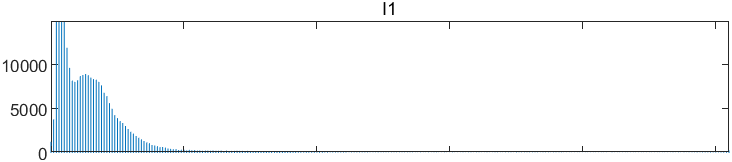
\includegraphics[width=1\columnwidth]{T2/result/hist1.png} 
	\caption{histgram of road1}
	\label{fig7}
\end{figure}
\begin{figure}[H]
 
	\centering
	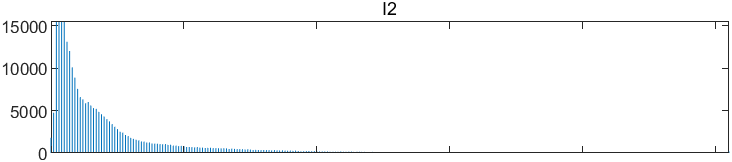
\includegraphics[width=1\columnwidth]{T2/result/hist2.png} 
	\caption{histgram of road2}
	\label{fig8}
\end{figure}
\begin{figure}[H]
 
	\centering
	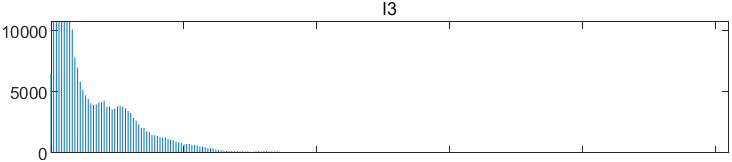
\includegraphics[width=1\columnwidth]{T2/result/hist3.png} 
	\caption{histgram of road3}
	\label{fig9}
\end{figure}
\subsection*{Answer} 

The three images above are the histograms of the three origin images grayscale values. We can see that the contrast of the picture is very low, The components of the histogram are concentrated at the low (dark) end of the gray level, and the width is narrow, and the distribution of the pixels is uneven.\\
In the histograms of road1 the grayscale values are concentrated at the low( dark) levels. There are two peaks.\\
In the histograms of road2 the grayscale values are concentrated at the low( dark) levels. There is only one peak.\\
In the histograms of road3 the grayscale values are concentrated at the low( dark) levels. There are one top peak and a few short peaks.\\My Matlab code is followed and is saved as \textbf{a.m}.
\begin{lstlisting}
	clc,clear;
	I1=imread("hw1_dark_road_1.jpg");
	I2=imread("hw1_dark_road_2.jpg");
	I3=imread("hw1_dark_road_3.jpg");
	figure('name','histogram','NumberTitle','off');
	subplot(3,1,1);
	imhist(I1);         %display the origin image
	title("I1");        
	subplot(3,1,2);
	imhist(I2);         %display the origin hist
	title("I2")
	subplot(3,1,3);
	imhist(I3);         %display the origin hist
	title("I3")
\end{lstlisting}

\begin{problem}
	b)  Apply global histogram equalization to the original image(MATLAB function: histeq is not allowed; just
	implement it by yourself and compare yours with Matlab’s ’histeq’). Display and submit the modified image. Plot
	and submit the histogram of the modified images grayscale values. Comment on visually desirable/undesirable
	regions in the modified image.
\end{problem}
\begin{figure}[H]
 
	\centering
	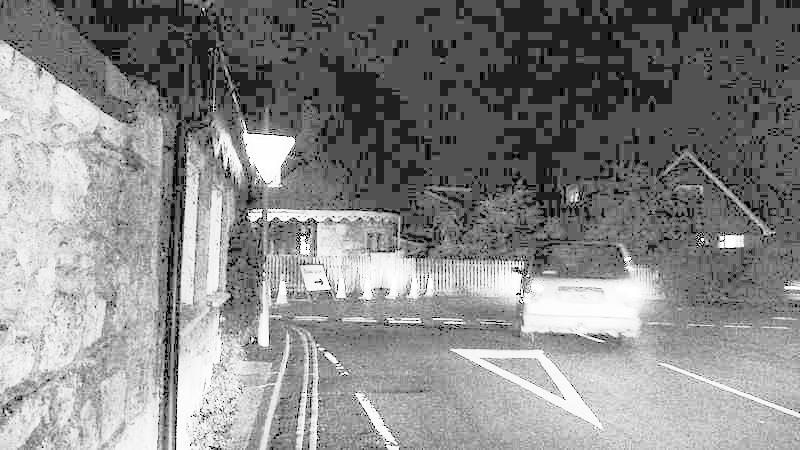
\includegraphics[width=1\columnwidth]{T2/result/I1_myglobal.jpg} 
	\caption{image of road1 after apply global histogram equalization}
	\label{fig10}
\end{figure}
\begin{figure}[H]
 
	\centering
	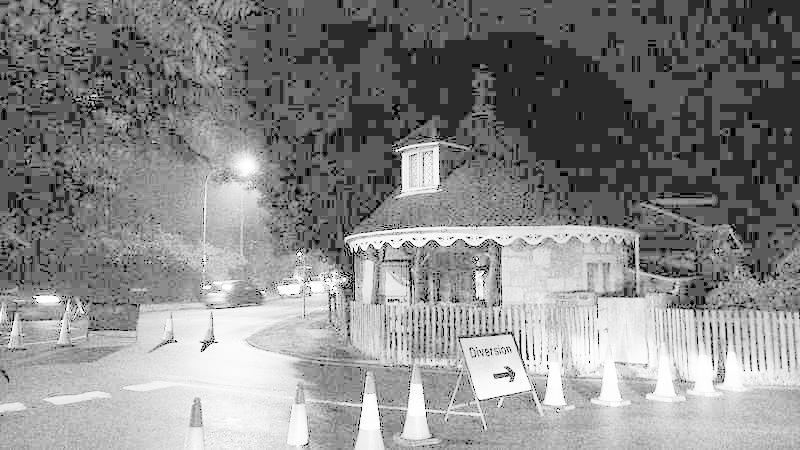
\includegraphics[width=1\columnwidth]{T2/result/I2_myglobal.jpg} 
	\caption{image of road2 after apply global histogram equalization}
	\label{fig11}
\end{figure}
\begin{figure}[H]
 
	\centering
	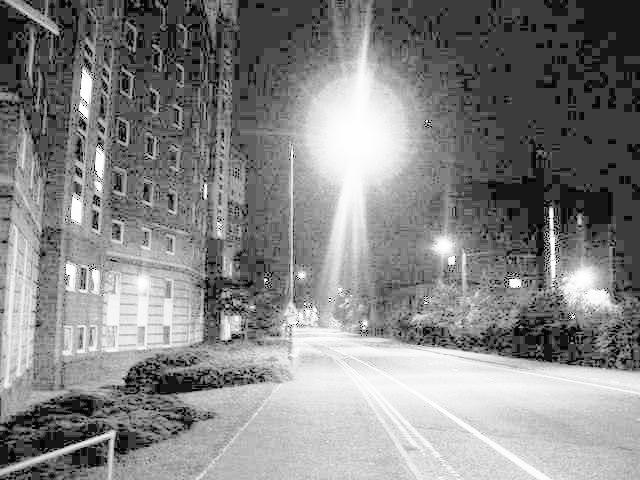
\includegraphics[width=1\columnwidth]{T2/result/I3_myglobal.jpg} 
	\caption{image of road3 after apply global histogram equalization}
	\label{fig12}
\end{figure}
\begin{figure}[H]
 
	\centering
	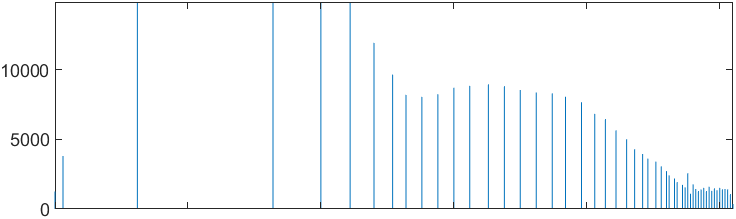
\includegraphics[width=1\columnwidth]{T2/result/hist1_myglobal.png} 
	\caption{histogram of road1 after apply global histogram equalization}
	\label{fig13}
\end{figure}
\begin{figure}[H]
 
	\centering
	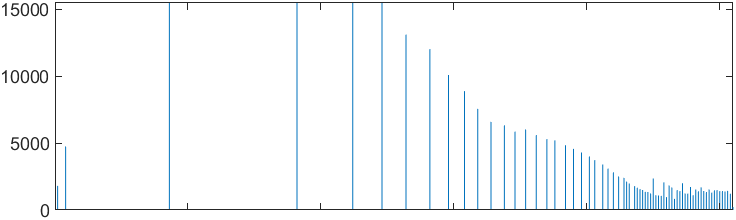
\includegraphics[width=1\columnwidth]{T2/result/hist2_myglobal.png} 
	\caption{histogram of road2 after apply global histogram equalization}
	\label{fig14}
\end{figure}
\begin{figure}[H]
 
	\centering
	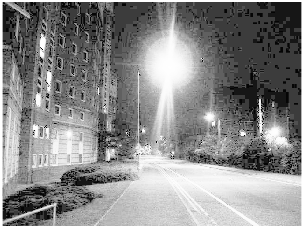
\includegraphics[width=1\columnwidth]{T2/result/hist3_myglobal.png} 
	\caption{histogram of road3 after apply global histogram equalization}
	\label{fig15}
\end{figure}
\begin{figure}[H]
 
	\centering
	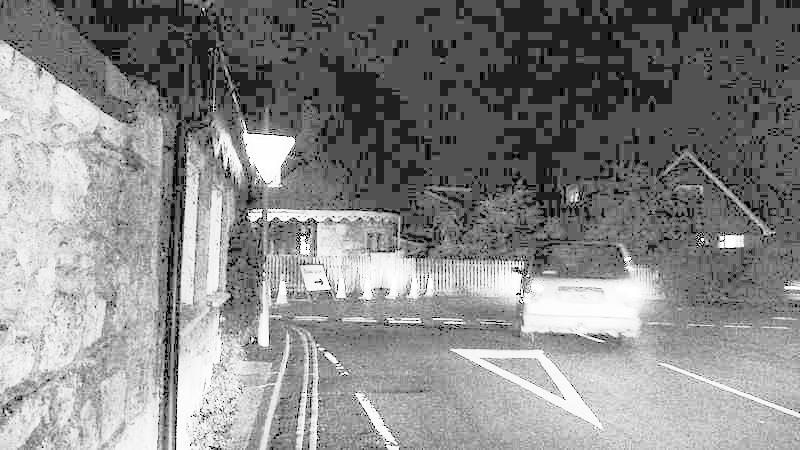
\includegraphics[width=1\columnwidth]{T2/result/I1_global.jpg} 
	\caption{image of road1 after apply histeq function}
	\label{fig16}
\end{figure}
\begin{figure}[H]
 
	\centering
	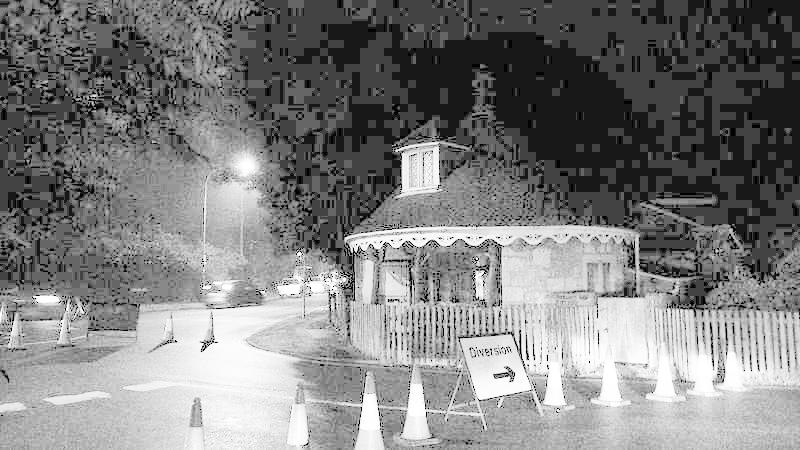
\includegraphics[width=1\columnwidth]{T2/result/I2_global.jpg} 
	\caption{image of road2 after apply histeq function}
	\label{fig17}
\end{figure}
\begin{figure}[H]
 
	\centering
	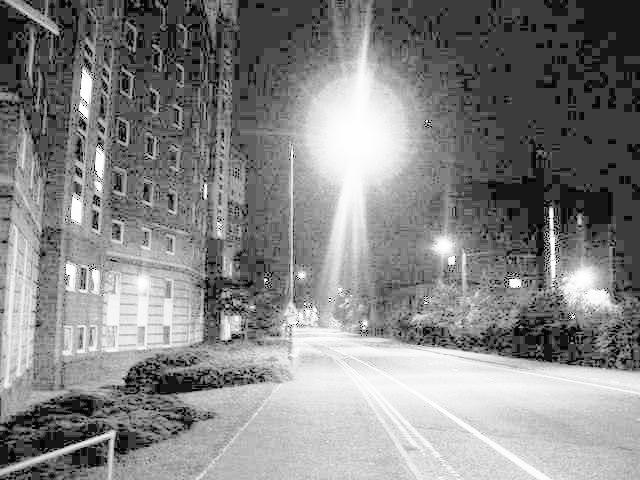
\includegraphics[width=1\columnwidth]{T2/result/I3_global.jpg} 
	\caption{image of road3 after apply histeq function}
	\label{fig18}
\end{figure}
\begin{figure}[H]
 
	\centering
	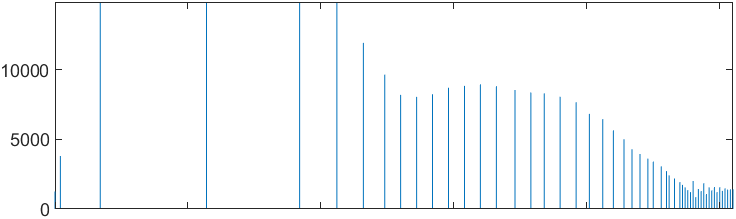
\includegraphics[width=1\columnwidth]{T2/result/hist1_global.png} 
	\caption{histogram of road1 after apply histeq function}
	\label{fig19}
\end{figure}
\begin{figure}[H]
 
	\centering
	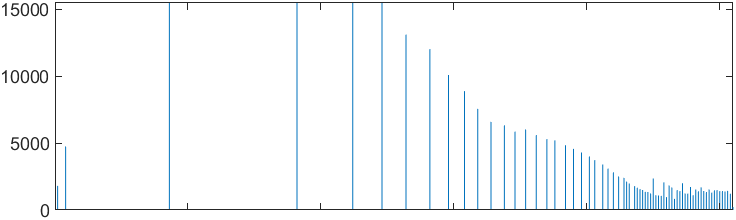
\includegraphics[width=1\columnwidth]{T2/result/hist2_global.png} 
	\caption{histogram of road2 after apply histeq function}
	\label{fig20}
\end{figure}
\begin{figure}[H]
 
	\centering
	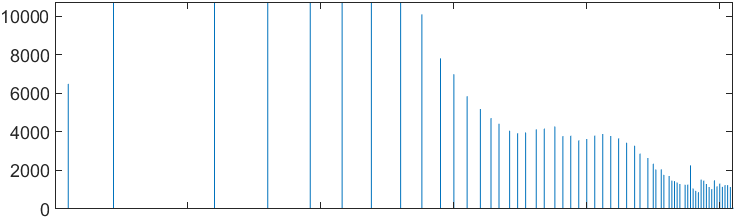
\includegraphics[width=1\columnwidth]{T2/result/hist3_global.png} 
	\caption{histogram of road3 after apply histeq function}
	\label{fig21}
\end{figure}
\subsection*{Answer} 
\textbf{Figure 10-12} are the images after applying global histogram equalization to the origin images.\\
We can see that The contrast of the image is greatly enhanced. For Example in the image of road1, we can see the wall, the lamp adn the car; in the image of road2, we can clearly see the car adn the house; in the picture of the road3, we can see the bushes and the department.\\
But there are many pacthes in the image because there are jumps between different grayscale values.\\
\textbf{Figure 10-12} are the images after applying histeq function in Matlab to the origin images, by comparision we can see that the results are almostly same.
My Matlab code is followed and is saved as \textbf{b.m} and \textbf{myhisteq.m}
\begin{lstlisting}
	%b.m
	clc,clear;
	I1=imread("hw1_dark_road_1.jpg");
	I2=imread("hw1_dark_road_2.jpg");
	I3=imread("hw1_dark_road_3.jpg");
	I1_process=myhisteq(I1);
	I2_process=myhisteq(I2);
	I3_process=myhisteq(I3)
	I1_process_2=histeq(I1,256);
	I2_process_2=histeq(I2,256);
	I3_process_2=histeq(I3,256);

	figure('name','road1自定义全局直方图均衡后的图片','NumberTitle','off');

	subplot(2,1,1);
	imshow(I1_process);         %display the MY process image
	imwrite(I1_process,"result/I1_myglobal.jpg","jpg");
			
	subplot(2,1,2);
	imhist(I1_process);         %display the MY process hist

	figure('name','road2自定义全局直方图均衡后的图片','NumberTitle','off');

	subplot(2,1,1);
	imshow(I2_process);         %display the MY process image
	imwrite(I2_process,"result/I2_myglobal.jpg","jpg");
			
	subplot(2,1,2);
	imhist(I2_process);         %display the MY process hist

	figure('name','road3自定义全局直方图均衡后的图片','NumberTitle','off');

	subplot(2,1,1);
	imshow(I3_process);         %display the MY process image
	imwrite(I3_process,"result/I3_myglobal.jpg","jpg");
			
	subplot(2,1,2);
	imhist(I3_process);         %display the MY process hist

	figure('name','road1全局直方图均衡后的图片','NumberTitle','off');

	subplot(2,1,1);
	imshow(I1_process_2);         %display the process image
	imwrite(I1_process_2,"result/I1_global.jpg","jpg");
			
	subplot(2,1,2);
	imhist(I1_process_2);         %display the process hist

	figure('name','road2全局直方图均衡后的图片','NumberTitle','off');

	subplot(2,1,1);
	imshow(I2_process_2);         %display the process image
	imwrite(I2_process_2,"result/I2_global.jpg","jpg");
			
	subplot(2,1,2);
	imhist(I2_process_2);         %display the process hist

	figure('name','road3全局直方图均衡后的图片','NumberTitle','off');

	subplot(2,1,1);
	imshow(I3_process_2);         %display the process image
	imwrite(I3_process_2,"result/I3_global.jpg","jpg");
			
	subplot(2,1,2);
	imhist(I3_process_2);         %display the process hist

\end{lstlisting}
\begin{lstlisting}
	%myhisteq.m
	function I_process = myhisteq(I)
	[height,width]=size(I);  %计算图片的宽和高

	r=zeros(1,256);           %用来存储之前每个灰度级处像素点的个数
	for i=1:height
		for j=1:width
			r(I(i,j)+1)=r(I(i,j)+1)+1;%统计每个灰度级处像素点的个数
		end
	end

	s=zeros(1,256);
	s(1)=r(1);
	for i=2:256
		s(i)=s(i-1)+r(i);        %对应书上公式计算只不过这里只算了CDF
	end

	for i=1:256
		s(i)=floor(255*s(i)/(height*width));        %对应书上公式,这里L-1取255
	end

	I_process=I;
	for i=1:height
	for j=1:width
		I_process(i,j)=s(I(i,j)+1);   %对每点处的灰度值进行映射
	end
	end
	end
\end{lstlisting}
\begin{problem}
	c)  Apply locally adaptive histogram equalization to the original image. Display
	and submit the modified image. Plot and submit the histogram of the modified images grayscale values. Choose
	and report the number of tiles and the clipping limit for attaining higher contrast while avoiding the generation
	of noisy regions and the amplification of nonuniform lighting effects. Comment on the subjective quality of the
	modified image compared to the result in (b).
\end{problem}
\begin{figure}[H]
 
	\centering
	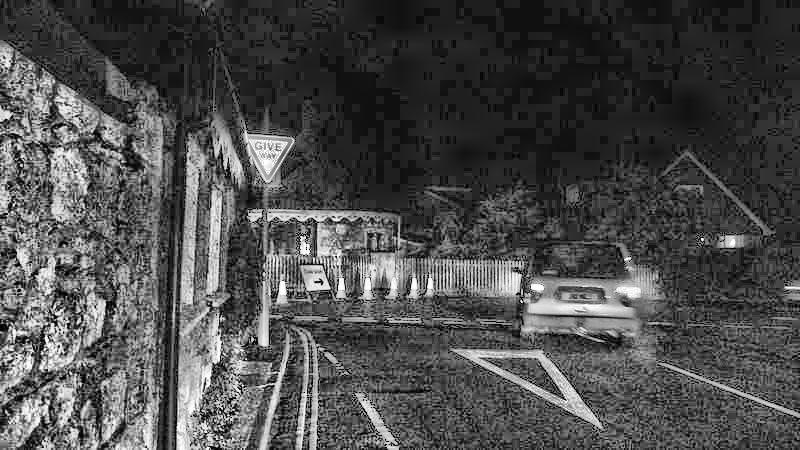
\includegraphics[width=1\columnwidth]{T2/result/I1_local.jpg} 
	\caption{image of road1 after apply local adaptive histogram equalization}
	\label{fig16}
\end{figure}
\begin{figure}[H]
 
	\centering
	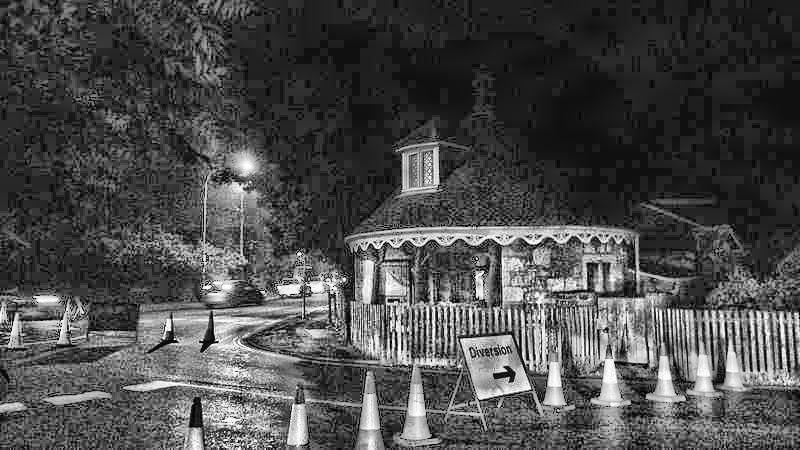
\includegraphics[width=1\columnwidth]{T2/result/I2_local.jpg} 
	\caption{image of road2 after apply local adaptive histogram equalization}
	\label{fig17}
\end{figure}
\begin{figure}[H]
 
	\centering
	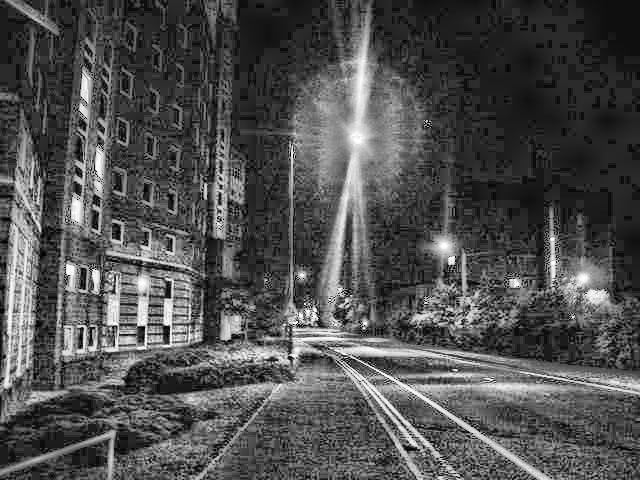
\includegraphics[width=1\columnwidth]{T2/result/I3_local.jpg} 
	\caption{image of road3 after apply local adaptive histogram equalization}
	\label{fig18}
\end{figure}
\begin{figure}[H]
 
	\centering
	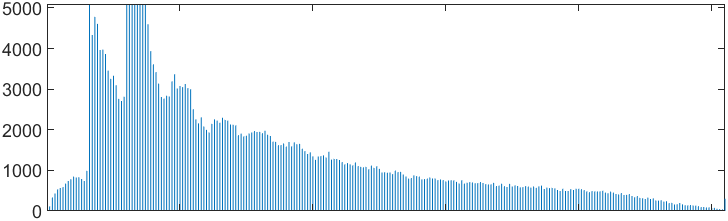
\includegraphics[width=1\columnwidth]{T2/result/hist1_local.png} 
	\caption{histogram of road1 after apply local adaptive histogram equalization}
	\label{fig19}
\end{figure}
\begin{figure}[H]
 
	\centering
	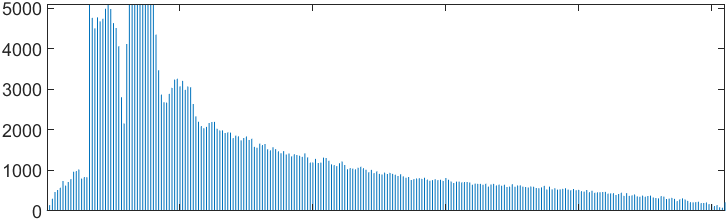
\includegraphics[width=1\columnwidth]{T2/result/hist2_local.png} 
	\caption{histogram of road2 after apply local adaptive histogram equalization}
	\label{fig20}
\end{figure}
\begin{figure}[H]
 
	\centering
	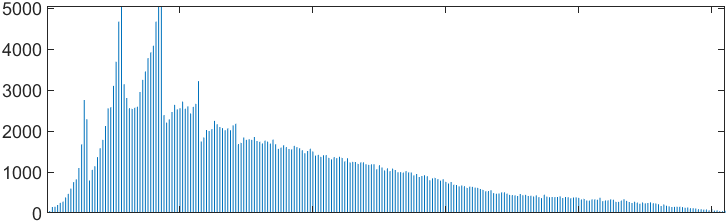
\includegraphics[width=1\columnwidth]{T2/result/hist3_local.png} 
	\caption{histogram of road3 after apply local adaptive histogram equalization}
	\label{fig21}
\end{figure}
\subsection*{Answer} 
\textbf{Figure 16-18} are the images after applying local adaptive histogram equalization to the origin images. We can see that the effect is much better than the case using global histgram equalization, There are not much patches, which makes us feel we can see more details in the images.\\
In the image of road1: tiles = 25*25, clipping limit =0.05;\\
In the image of road2: tiles = 25*25, clipping limit =0.05;\\
In the image of road3: tiles = 25*25, clipping limit =0.05;\\
My Matlab code is followed and is saved as \textbf{c.m}.
\begin{lstlisting}
	clc,clear;
	I1=imread("hw1_dark_road_1.jpg");
	I2=imread("hw1_dark_road_2.jpg");
	I3=imread("hw1_dark_road_3.jpg");

	I1_process=adapthisteq(I1,'NumTiles',[25 25],'ClipLimit',0.05);
	I2_process=adapthisteq(I2,'NumTiles',[25 25],'ClipLimit',0.05); 
	I3_process=adapthisteq(I3,'NumTiles',[25 25],'ClipLimit',0.05); 

	figure('name','road1局部适应直方图均衡后的图片','NumberTitle','off');

	subplot(2,1,1);
	imshow(I1_process);         %display the process image
	imwrite(I1_process,"result/I1_local.jpg","jpg");
			
	subplot(2,1,2);
	imhist(I1_process);         %display the process hist

	figure('name','road2局部适应直方图均衡后的图片','NumberTitle','off');

	subplot(2,1,1);
	imshow(I2_process);         %display the process image
	imwrite(I2_process,"result/I2_local.jpg","jpg");
			
	subplot(2,1,2);
	imhist(I2_process);         %display the process hist

	figure('name','road3局部适应直方图均衡后的图片','NumberTitle','off');

	subplot(2,1,1);
	imshow(I3_process);         %display the process image
	imwrite(I3_process,"result/I3_local.jpg","jpg");
			
	subplot(2,1,2);
	imhist(I3_process);         %display the process hist
\end{lstlisting}
\begin{problem}
	d)  Apply a $\gamma$-nonlinearity mapping to each image to perform contrast enhancement, show the new image, and
	submit the displayed image. For each image, find and report a value of $\gamma$ that allows you to see more details.
	
\end{problem}
\begin{figure}[H]
 
	\centering
	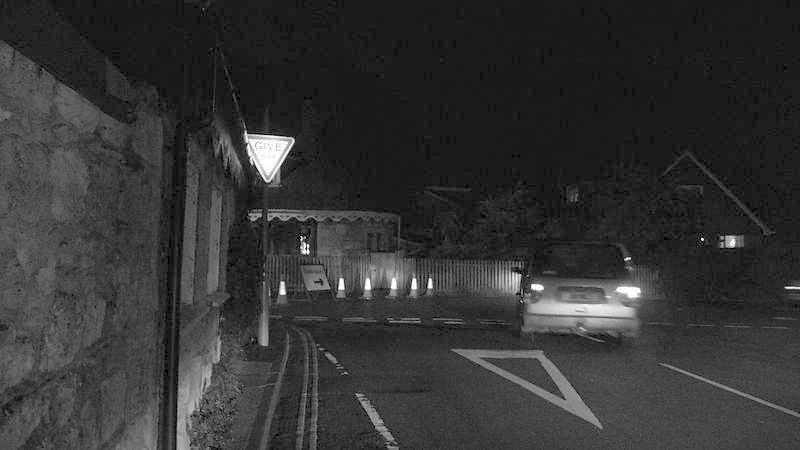
\includegraphics[width=1\columnwidth]{T2/result/I1_gama.jpg} 
	\caption{image of road1 after apply $\gamma$-nonlinearity mapping}
	\label{fig22}
\end{figure}
\begin{figure}[H]
 
	\centering
	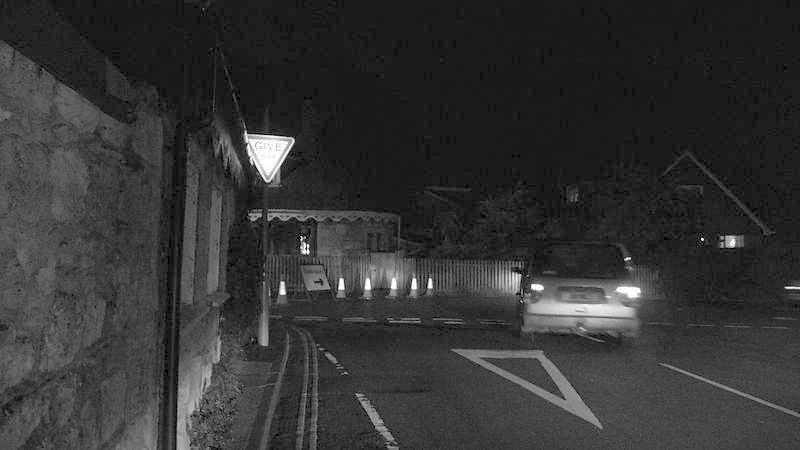
\includegraphics[width=1\columnwidth]{T2/result/I2_gama.jpg} 
	\caption{image of road2 after apply $\gamma$-nonlinearity mapping}
	\label{fig23}
\end{figure}
\begin{figure}[H]
 
	\centering
	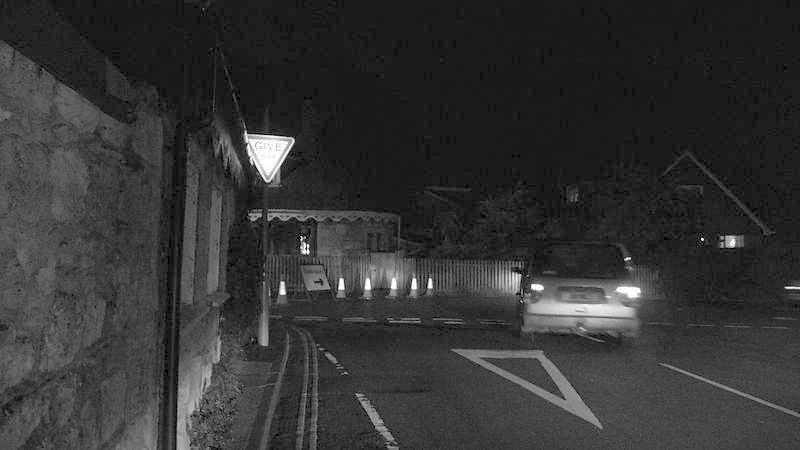
\includegraphics[width=1\columnwidth]{T2/result/I3_gama.jpg} 
	\caption{image of road3 after apply $\gamma$-nonlinearity mapping}
	\label{fig24}
\end{figure}
\subsection*{Answer}
The images above are processed images after apply $\gamma$-nonlinearity mapping, the value of $\gamma$ is 0.4., $c$ is 1.\\
I try from 0.1 to 1 and compare the results. I find the 0.4 is the best, so I only report this.
My Matlab code is followed and is saved as \textbf{d.m} and \textbf{gama.m}
\begin{lstlisting}
	%d.m
	clc,clear;
	I1=imread("hw1_dark_road_1.jpg");
	I2=imread("hw1_dark_road_2.jpg");
	I3=imread("hw1_dark_road_3.jpg");

	I1_process=gama(im2double(I1),0.5);
	figure('name','幂律变换后的图片','NumberTitle','off');
	imshow(I1_process);         %display the process image
	imwrite(I1_process,"result/I1_gama.jpg","jpg");

	I2_process=gama(im2double(I1),0.5);
	figure('name','幂律变换后的图片','NumberTitle','off');
	imshow(I2_process);         %display the process image
	imwrite(I2_process,"result/I2_gama.jpg","jpg");

	I3_process=gama(im2double(I1),0.5);
	figure('name','幂律变换后的图片','NumberTitle','off');
	imshow(I3_process);         %display the process image
	imwrite(I3_process,"result/I3_gama.jpg","jpg");
\end{lstlisting}
\begin{lstlisting}
	%gama.m
	function process_img = gama(img,x)
    
    process_img=img.^x;

	end
\end{lstlisting}
\end{document}
